\chapter{Why You Need To Learn Sales Before You Start a Company}

The chapter opens with the answer before it gives us the formal question. That order should be preserved, because the speaker begins not with biography or technique but with a boundary: there are things one can look up, and there are things one can only undergo. What follows is an explanation of how early sales work becomes training for company-building. To keep the mechanism clear without pretending that the source is a blackboard lecture, we will use a small amount of notation as a disciplined summary of the transcript rather than as quoted formalism.

\section{The Opening Boundary}

The first claim is abrupt and definitive: experience cannot be Googled. One cannot retrieve it as one retrieves information. One has to go through it. The chapter should therefore begin with the distinction between searchable content and lived passage:
\begin{equation}
E_{\mathrm{lived}} \neq E_{\mathrm{textbook}}.
\end{equation}
Here \(E_{\mathrm{lived}}\) denotes direct contact with real situations, while \(E_{\mathrm{textbook}}\) denotes what may be learned from description, instruction, or secondhand advice.

This is already more than a slogan. It tells us what kind of argument is coming. The speaker is not saying that books, advice, or verbal training are useless. He is saying that there is a class of competence whose decisive component arrives only under contact with reality. We are meant to hold that distinction in mind while the interviewer then backs up and asks the practical business question.

\section{The Question: How Does Sales Turn into Ownership?}

Only after the cold open do we hear the frame. Early in his career, the speaker was primarily in sales. How did the skills learned there help him own a company at such a young age? That question is important because it prevents the discussion from floating off into vague praise of resilience. We are being asked for a translation rule from one domain to another: from selling to building.

\begin{definition}
For editorial convenience, we introduce the following symbols:
\begin{align}
T &:= \{\text{tricks},\ \text{phrases},\ \text{appearance}\}, \\
S &:= \text{practical sales skill}, \\
N &:= \text{repeated negative encounters}, \\
A &:= \text{stability of attitude under pressure}, \\
M &:= \text{quality of message delivery under pressure}, \\
V &:= \text{variation in the people one must address}.
\end{align}
These are not lecture-given symbols. They simply allow us to keep the transcript's causal structure visible on the page.
\end{definition}

The answer does not come back as a list of tactics for running a company. Instead, it begins by separating what may be taught quickly from what only forms slowly.

\section{What Instruction Can Give Us}

The speaker concedes a good deal at the outset. One can be taught tricks. One can be taught what to say. One can even learn to present oneself well. In our shorthand,
\begin{equation}
T=\{\text{tricks},\ \text{phrases},\ \text{appearance}\}.
\end{equation}
This concession matters. It prevents the later claim from becoming anti-intellectual or careless. The lecture does not deny that there are teachable elements in sales. It denies that these elements exhaust the skill.

That is the reason for the next step:
\begin{equation}
S \neq T.
\end{equation}
To know lines is not yet to know how to sell. To dress well is not yet to know how to remain effective when the interaction becomes adversarial. At this point the lecture tightens. We are no longer discussing polish in the abstract; we are moving toward the conditions under which polish is tested.

\subsection{Question \& Answer}

Why does a textbook fail, even when it contains useful advice?

Because the missing term is not verbal content but lived stress. The transcript answers this question by escalation rather than by abstract definition: being told no, then told no again, then cursed at, then screamed at, and nevertheless having to keep the same attitude and still deliver the message the right way. That is why a cautious summary of the lecture's asymmetry is
\begin{equation}
E_{\mathrm{textbook}} \not\to S,
\qquad
E_{\mathrm{lived}} \to S.
\end{equation}
The arrows are causal, not quantitative. The point is simply that description may prepare us, but it does not complete us.

We should notice the rhythm here. The speaker first grants the limited truth of instruction, and only then does he deny its sufficiency. That order is part of the lecture's precision.

\section{Rejection as the Training Mechanism}

Now the real mechanism appears. The lecture does not speak of hardship in a single generic phrase. It piles it up. There is rejection, then repeated rejection, then open hostility. And at each stage the demand is the same: keep the same attitude, and still deliver the message properly. This is where the interview becomes analytically sharp.

If we let \(S_k\) denote the skill state after the \(k\)-th meaningful encounter, then a careful process summary is
\begin{align}
S_{k+1} &= S_k + \Delta S_k, \\
\Delta S_k &= \Phi(N_k,A_k,M_k,V_k).
\end{align}
Here \(\Phi\) is not a measurable law. It is only a reminder that the gain in skill during one encounter depends on the pressure faced, the steadiness of attitude, the quality of delivery, and eventually the diversity of the audience.

The logic of the update can be written step by step.
\begin{enumerate}
\item We begin with preparation: a repertoire of lines, tricks, and surface presentation, summarized by \(T\).
\item We then enter a live encounter in which resistance is possible and often actual.
\item The encounter tests whether attitude remains stable; this is the variable \(A_k\).
\item At the same time, the encounter tests whether the message still comes out correctly; this is the variable \(M_k\).
\item If pressure is real and both attitude and delivery hold together well enough, then \(\Delta S_k>0\).
\item Repetition of such encounters turns isolated effort into embodied competence.
\end{enumerate}

This is the point at which the line ``no after no after no'' does real work. It is not ornamental repetition. It marks iteration. The lecture is telling us that competence is not transferred in one step; it is accumulated by surviving the same basic test many times without losing composure or clarity.

\begin{figure}[h]
\centering
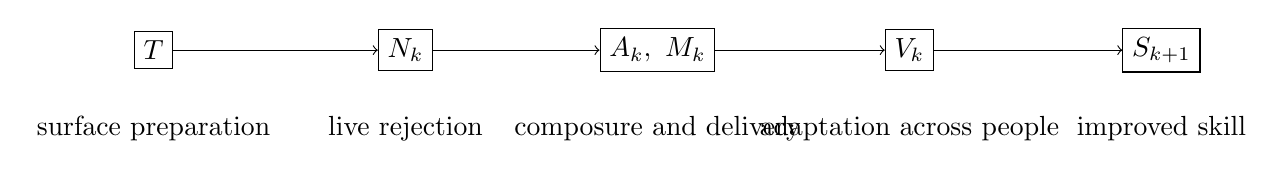
\begin{tikzpicture}
\node[draw, rectangle] (t) at (0,0) {$T$};
\node[draw, rectangle] (n) at (3.2,0) {$N_k$};
\node[draw, rectangle] (am) at (6.4,0) {$A_k,\ M_k$};
\node[draw, rectangle] (v) at (9.6,0) {$V_k$};
\node[draw, rectangle] (s) at (12.8,0) {$S_{k+1}$};

\draw[->] (t) -- (n);
\draw[->] (n) -- (am);
\draw[->] (am) -- (v);
\draw[->] (v) -- (s);

\node at (0,-1) {surface preparation};
\node at (3.2,-1) {live rejection};
\node at (6.4,-1) {composure and delivery};
\node at (9.6,-1) {adaptation across people};
\node at (12.8,-1) {improved skill};
\end{tikzpicture}
\end{figure}

The figure is an editorial schematic, not a recovered lecture image. It is included only to keep the transcript's sequence visible: preparation, rejection, composure, adaptation, improvement.

\section{Why Variety Makes the Skill Broader}

After the sequence of hostility, the lecture does not stop. It adds another dimension. Sales forces one to communicate with different ethnicities, different backgrounds, different ages, different experiences. This is a genuine extension of the argument. We are not merely learning to withstand pressure. We are learning to adjust across many human contexts.

That is why the most compact summary of the chapter's mechanism is
\begin{equation}
S = f(N,A,M,V).
\end{equation}
The notation is editorial, but the ingredients are transcript-backed. The speaker has already identified repeated resistance, stable attitude, proper delivery, and wide variation in audience as the conditions under which the skill grows.

We may then write the concluding tendency in the mildest possible way:
\begin{equation}
N \uparrow,\quad V \uparrow
\qquad \Longrightarrow \qquad
S \uparrow,
\end{equation}
provided the salesperson continues to preserve attitude and message under stress. The point is not that this is a calibrated theorem. The point is that the lecture closes on an inevitability claim: under these conditions, one has no choice but to get better.

That final phrase is important. Improvement is not presented as inspiration, self-help, or positive thinking. It is presented as the natural consequence of exposure. And from there the entrepreneurial translation is straightforward. A person who has learned to keep composure under rejection, and to speak effectively across many kinds of people, carries into company-building a skill that is deeper than technique alone.

\section{From Sales Skill to Founding Capacity}

We can now return to the interviewer's original question. How does sales help one own a company young? The answer is not that sales provides a secret script for entrepreneurship. It is that sales creates a disciplined encounter with resistance. It teaches us how to absorb negative feedback without collapse, how to keep the message intact while emotion is running against us, and how to adapt when the person in front of us is not like the last person in front of us.

Seen this way, the transfer from sales to ownership is not mysterious. Founding a company requires persuasion, steadiness, repetition, and the ability to communicate across different kinds of people: customers, partners, employees, and investors. The lecture does not list those roles explicitly, and we should not overextend it, but the structure of the transfer is plain. The school is sales; the acquired capacity is broader.

\section{Summary}

The lecture proceeds in a clean order, and the chapter should end by preserving that order. First comes the boundary: experience cannot be Googled. Then comes the business question: how does sales translate into company ownership? Then comes the concession that tricks, phrases, and appearance can indeed be taught. Only after that does the decisive claim arrive: such things are not enough, because real skill is formed by passing through rejection while keeping both attitude and message intact. The lecture then widens the frame from repeated rejection to repeated contact with many different kinds of people, and it closes by insisting that under such conditions improvement is nearly forced.

The result is a compact but serious theory of formation. Sales matters here not as a bag of lines but as a repeated encounter with resistance and variety. That is why it becomes preparation for building: one who has gone through that training has learned something no search bar can provide.